\fancyhead[LO, RE] {Studio delle Tecnologie}
\section{Studio delle Tecnologie}
\subsection{Stealth 3000}
La maggior parte delle aziende tessili di larga scala in Italia utilizza un ERP specifico, Stealth 3000, sviluppato dall'azienda italiana Dedagroup.\\
In quanto ERP connette tutti gli applicativi utilizzati dall'azienda, oltre ad essere un gestionale disegnato specificatamente per il mercato della moda. \\
Si tratta di un'applet Java, accessibile solo internamente all'azienda da Internet Explorer e Firefox.\\
Di seguito verrà illustrato il funzionamento di Stealth 3000 negli ambiti che sono stati toccati dal progetto CRM, che sono solo una minima parte di quanto offerto dall'ERP. Gli ambiti in questione sono i Soggetti, ovvero i clienti in generale, e le loro condizioni commerciali, gli oggetti e le loro classificazioni, ovvero gli articoli che vengono venduti ed infine i listini di vendita.\\
Tutti i contenuti anagrafici dei dati rappresentati sono fittizi, ottenuti dai manuali d'uso a scopo formativo.

\subsubsection{Soggetto}
Sono una qualunque entità fisica, giuridica, gestionale, organizzativa con cui l'azienda intrattiene rapporti di business.\\
Esempi di Soggetti sono: Clienti, Fornitori, Agenti,Terzisti, Importatori, Distribution Centers, Reparti interni.\\
L'archivio dei soggetti ne contiene i dati anagrafici fissi nel tempo (Ragione Sociale, Partita IVA, Indirizzo, ecc). Il soggetto ha una lista di indirizzi associati che ne definiscono punti di riferimento, ad esempio potrebbe avere un indirizzo di fatturazione ed un indirizzo di spedizione diversi tra loro.\\
Il soggetto può avere contemporaneamente più \textbf{Ruoli}; Esso rappresenta il tipo di rapporto che il Soggetto ha con l'Azienda, e può essere di tre tipi: \textbf{Cliente}, \textbf{Fornitore} o \textbf{Agente}. A seconda del ruolo ci sono differenti \textbf{Condizioni Commerciali}.
Di seguito la form di anagrafica Soggetto vista da Stealth 3000:
\newpage
\begin{figure}[!h]
\thispagestyle{empty}
\centering
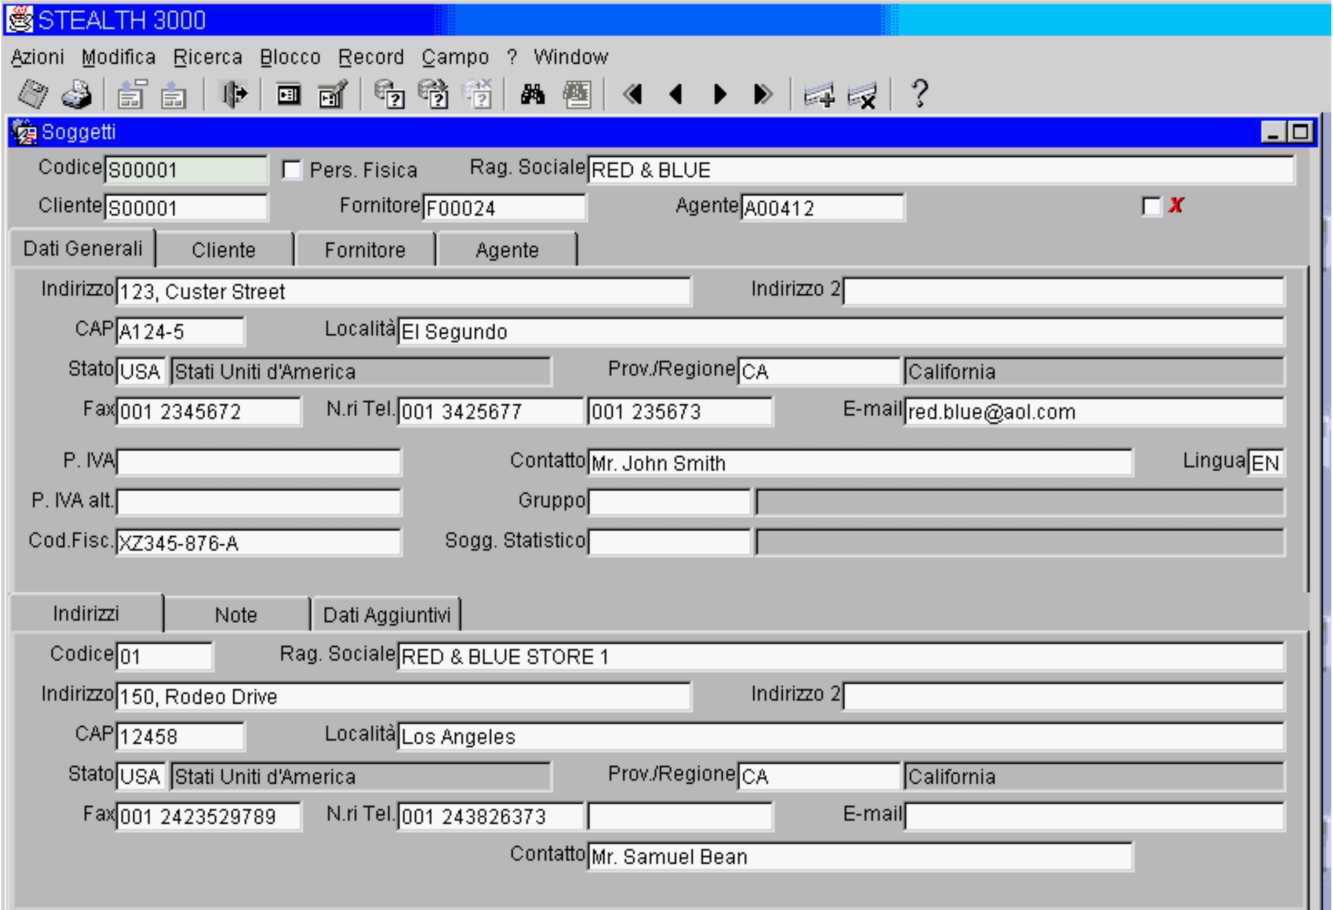
\includegraphics[scale=0.45]{img/SogAnag.png}
\caption{Anagrafica Soggetti}
\end{figure}
\newpage
Dati di testata:
\begin{table}[!h]
	\begin{center}
	
	\begin{tabular}{| c | c |}
	\hline
	\textbf{Dato} & \textbf{Descrizione} \\ \hline
	Codice & \begin{tabular}{@{}c@{}@{}@{}@{}@{}}  Codice Soggetto: in fase di creazione il codice\\ viene attribuito automaticamente all’uscita\\ del campo da un numeratore pubblico \\ma può essere forzato dall’utente.\\ Il sistema effettuerà in automatico un controllo\\ di unicità del codice all’interno del database.\end{tabular} \\ \hline

	Persona Fisica &  \begin{tabular}{@{}c@{}@{}@{}}   Flag che indica che il soggetto è una persona fisica\\ anzichè giuridica, per cui il campo della\\ Ragione sociale dovrà essere sostituito\\ dall’inserimento di Cognome e Nome.\end{tabular}\\ \hline

	Ragione Sociale & Descrizione della missione aziendale.\\ \hline
	
	Cliente &  \begin{tabular}{@{}c@{}@{}@{}@{}}  Codice corrispondente al ruolo cliente (se esistente)\\  del soggetto. Il codice sarà assegnato\\  in automatico alla generazione del ruolo\\ ed il campo presente servirà per ricerche \\mirate ai soli ruoli cliente.\end{tabular}\\ \hline
Fornitore &  \begin{tabular}{@{}c@{}@{}@{}@{}}  Codice corrispondente al ruolo Fornitore (se esistente)\\  del soggetto. Il codice sarà assegnato\\  in automatico alla generazione del ruolo\\ ed il campo presente servirà per ricerche mirate \\ai soli ruoli Fornitore.\end{tabular}\\ \hline
Agente &  \begin{tabular}{@{}c@{}@{}@{}@{}}  Codice corrispondente al ruolo agente (se esistente)\\  del soggetto. Il codice sarà assegnato\\  in automatico alla generazione del ruolo\\ ed il campo presente servirà per ricerche \\mirate ai soli ruoli agente.\end{tabular}\\ \hline

\end{tabular} 
	\caption{Soggetti: Dati di testata}
\end{center}
\end{table}
\newpage
Dati Generali:
\begin{longtable}{| c | c |}%{| p{.20\textwidth} | p{.80\textwidth} |}
	
	\hline
	\textbf{Dato} & \textbf{Descrizione} \\ \hline
	Indirizzo & \begin{tabular}{@{}c@{}@{}@{}} Primo campo dell’indirizzo: è un campo\\ ad inserimento di testo libero, lungo fino\\ a 50 caratteri ed è il campo principale di\\ esposizione dell’indirizzo sintetico del cliente.\end{tabular} \\ \hline

	Indirizzo 2 &  \begin{tabular}{@{}c@{}@{}@{}@{}@{}}  Secondo campo dell’indirizzo: è un campo\\ aggiuntivo di testo libero che\\ viene utilizzato quando il primo sia\\ insufficiente oppure si voglia riportare dati\\ su una riga diversa dell’etichetta completa\\ del soggetto.\end{tabular}\\ \hline

	CAP &  \begin{tabular}{@{}c@{}@{}@{}@{}@{}} Indicazione del Codice di avviamento postale\\ della nazione a cui appartiene il soggetto.\\ L’obbligatorietà di questo campo è\\ determinata da un parametro della tabella\\ stati, in corrispondenza dello\\ stato che sarà indicato più sotto.\end{tabular}\\ \hline

	Località &  \begin{tabular}{@{}c@{}@{}@{}} Città, paese, frazione di identificazione\\ dell’indirizzo. In molte visualizzazioni\\ sintetiche dei codici soggetti\\ accompagna la ragione sociale.\end{tabular}\\ \hline

	Stato &  \begin{tabular}{@{}c@{}@{}@{}@{}@{}} Codice corrispondente nella tabella degli\\ stati a cui sono collegati molti controlli\\ sull’inserimento degli altri dati nella form\\ come Codice Fiscale, Partita IVA, Prov/Reg.,\\ Formato del codice Bancario,\\ Valuta di default.\end{tabular}\\ \hline

	Prov/Regione &  \begin{tabular}{@{}c@{}@{}@{}}   Valore che può essere reso obbligatorio\\ per lo stato inserito con controllo di\\ relazionalità con la tabella collegata\\ a quella degli stati.\end{tabular}\\ \hline

	Fax– N.Tel–E-mail &  \begin{tabular}{@{}c@{}@{}@{}}  Dati di libero inserimento che potranno\\ essere presentati su altre form,\\ stampe oppure essere utilizzati da\\ procedure personalizzate.\end{tabular}\\ \hline

	P.IVA &  \begin{tabular}{@{}c@{}@{}@{}@{}}  Codice di Partita IVA del soggetto.\\ È obbligatoria e all’uscita del campo attiva\\ i controlli formali sul codice (secondo il paese\\ di appartenenza) e di codici duplicati già\\ presenti nel database (controllo non bloccante).\end{tabular}\\ \hline
	
	Contatto &  \begin{tabular}{@{}c@{}}  Campo libero di inserimento\\ dei dati utili all’utente.\end{tabular}\\ \hline

	Lingua &  \begin{tabular}{@{}c@{}@{}@{}}   Lingua di default per la gestione dei documenti\\ del soggetto, viene proposta in automatico\\ dalla tabella degli stati, ma può essere\\ modifica dall’utente.\end{tabular}\\ \hline
	
	P.IVA alt &  \begin{tabular}{@{}c@{}@{}@{}@{}}  Indicazione del codice di Partita IVA\\ internazionale che solitamente\\ è formata dal codice ISO dello stato\\ di appartenenza concatenato con il\\ codice di Partita Iva inserito nel campo precedente.\end{tabular}\\ \hline
	
	Codice Fiscale &  \begin{tabular}{@{}c@{}}  Può essere obbligatorio per lo stato\\ e per la natura fiscale del soggetto.\end{tabular}\\ \hline

	Gruppo &  \begin{tabular}{@{}c@{}} Codice di soggetto a cui il soggetto corrente\\ è legato da rapporti di gruppo.\end{tabular}\\ \hline

	Sogg. Statistico &  \begin{tabular}{@{}c@{}}Codice Soggetto a cui legare più soggetti\\ al fine di analisi statistiche raggruppate.\end{tabular}\\ \hline

	Società Intercompany &  \begin{tabular}{@{}c@{}@{}@{}@{}}   Codice societario assegnato al cliente\\ se appartiene al dominio delle società definite\\ “Intragruppo”. Questi soggetti avranno\\ particoli processi di trattamento\\ per i rapporti attivi e passivi.\end{tabular}\\ \hline
	
	\caption{Soggetti: Dati Generali}

\end{longtable}

\subsubsection{Condizioni di Vendita}
Di seguito vediamo la form delle Condizioni di Vendita (colloquialmente, Condizioni Commerciali) accessibili dalla schermata dei Soggetti in (figura 1).

%Figura Cond Comm

Tramite questa form è possibile gestire i dati di vendita del cliente con record multipli la cui chiave è: Anno/Stagione/Marchio/Tipologia di Vendita.\\
Con questa configurazione è possibile memorizzare per ogni cliente diverse configurazioni di dati per la vendita in dipendenza di diverse Stagioni e/o Marchi e/ Tipologie di vendita; nel caso in cui uno o più campi chiave siano vuoti il loro significato corrisponde a “tutte le ricorrenze corrispondenti”. Ad esempio nel caso (in figura) le condizioni di vendita sono nominalmente valide per tutte le stagioni, tutti i marchi e tutte le tipologie di vendita, mentre se fosse stato valorizzato l'anno/stagione, sarebbero state valide per tutti i marchi/tipologie di vendita di quel determinato anno/stagione.\\
Descrizione dei dati generali delle Condizioni di Vendita:

\begin{longtable}{| c | c |}%{| p{.20\textwidth} | p{.80\textwidth} |}
	
	\hline
	\textbf{Dato} & \textbf{Descrizione} \\ \hline
	Valuta & \begin{tabular}{@{}c@{}@{}} Valuta di defautl che sarà\\  proposta in tutti i documenti attivi\\ generati per il cliente di fatturazione.\end{tabular} \\ \hline  

	Tipo Listino &  \begin{tabular}{@{}c@{}@{}}  Codice del tipo listino che sarà utilizzato\\ per il reperimento dei prezzi nella\\generazione dei documenti attivi. \end{tabular}\\ \hline   

	Pagamento &  \begin{tabular}{@{}c@{}@{}} Codice di pagamento che sarà proposto\\di default per i documenti attivi generati\\ per il cliente quando questo è il cliente intestatario.\end{tabular}\\ \hline   

	Giorno Preferenziale &  \begin{tabular}{@{}c@{}@{}} Giorno del mese di preferenza per\\ le scadenze dei pagamenti che\\saranno generati al cliente.\end{tabular}\\ \hline  

	Contabilità &  \begin{tabular}{@{}c@{}@{}@{}@{}@{}} Questo flag determina quale tra le\\ condizioni di vendita inserite sarà\\ la fonte dei dati che saranno trasmessi al\\ sistema amministrativo. Per questa\\ ragione ci può essere una sola Condizione\\  di vendita con questo flag alzato.\end{tabular}\\ \hline     

	Inizio Fine In &  \begin{tabular}{@{}c@{}@{}@{}}   Tramite questa coppia di dati è possibile\\ stabilire due periodi dell’anno (Da Giorno/Mese\\ a Giorno/Mese) in cui le scadenze\\ di pagamento dovranno essere ricondotte\\  al Giorno/Mese indicato nela campo 'In'.\end{tabular}\\ \hline   

	Banca Cli. &  \begin{tabular}{@{}c@{}@{}}  Codice della tabella banche del Soggetto\\da utilizzare come banca trassata preferenziale\\ dei pagamenti del cliente di fatturazione.\end{tabular}\\ \hline   

	IBAN Cli. &  \begin{tabular}{@{}c@{}@{}} Codice IBAN (Diviso tra prefisso naz.-Cin)\\ e codice vero e proprio tra quelli disposti\\ nella tabella banche del Soggetto.\end{tabular}\\ \hline
	
	Banca di appoggio - IBAN &  \begin{tabular}{@{}c@{}@{}c@{}@{}c@{}@{}}  Codice della banca e IBAN del conto\\ corrente preferenziale sul quale appoggiare\\ i pagamenti del cliente. Nel caso di più linee\\  di credito dell’Azienda è possibile così pilotare\\  gli effetti da emettere presso l’Istituto \\  Bancario più conveniente per i \\  rapporti con la banca del Cliente. \end{tabular}\\ \hline 

	Agente &  \begin{tabular}{@{}c@{}}   Codice Agente abilitato al cliente corrente\\  per la stagione/Marchio/Tipo di vendita prescelti.\end{tabular}\\ \hline 

	Importatore &  \begin{tabular}{@{}c@{}@{}@{}@{}}  Flag che indica come il cliente sia\\  da considerare Importatore per cui l’emissione\\ del documento di vendita al cliente di\\  fatturazione dovrà essere riferito a\\ condizioni di vendita diverse da quelle\\ applicate ai clienti di destinazione. \end{tabular}\\ \hline    

	Classe Cl.–Eventi &  \begin{tabular}{@{}c@{}}  Codice di classe del cliente a cui può\\essere abilitato uno o più eventi di vendita.\end{tabular}\\ \hline  

	Label &  \begin{tabular}{@{}c@{}@{}@{}@{}@{}} Codice aggiuntivo dei prodotti che sarà \\aggiunto automaticamente alle righe ordini\\  in maniera da caratterizzare puntualmente\\  il fabbisogno, la disponibilità e relative\\ assegnazioni al cliente specifico (Forniture speciali). \end{tabular}\\ \hline   

	Cartellino &  \begin{tabular}{@{}c@{}} Codice aggiuntivo dall’uso \\ uguale al precedente. \end{tabular}\\ \hline  

	Sconti Comm. &  \begin{tabular}{@{}c@{}@{}}    Percentuali di sconto multiple, che\\ saranno applicate in cascata a tutti\\gli ordini di cui il cliente è intestatario. \end{tabular}\\ \hline  

	Provvigioni   &  \begin{tabular}{@{}c@{}@{}}     Percentuali di sconto multiple, che\\ saranno applicate in cascata \\all’agente abilitato al cliente.  \end{tabular}\\ \hline 

	\caption{Condizioni di Vendita: Dati Generali}

\end{longtable}

\subsubsection{Modelli}
Gli Oggetti nel package Stealth 3000 sono tutti i tipi di prodotto che possono essere gestiti come beni d’acquisto (materie prime e componenti di Distinta Base), acquistati e/o prodotti, gestiti a magazzino, venduti e così via. \\
Le anagrafiche Oggetti (Modello, Parte, Modello/Parte) sono gestite in due livelli: a livello di 'Gruppo', ovvero pubbliche a tutte le società e a livello 'Società', ovvero l'appartenenza è limitata alla stessa, che è l'unica in grado di apportare modifiche.\\
 La maggior parte dei dati delle anagrafiche sono a livello Pubblico, mentre solo alcuni dati di Vendita e Gestione sono a livello Società.

Il Modello (Style) è l’oggetto che descrive la forma generica con cui classificare i Prodotti da vendere (Abiti, Giacche, Gonne ecc...). Hanno taglie e misure ma non colori o tessuti associati, non si rappresentano oggetti fisici.\\ 
Il codice del Modello è una combinazione di caratteristiche anagrafiche, nello specifico [Codifica Anno/Stagione][Linea][Codice Modello][Variante] in rispettivamente 2, 3, 5 e 2 caratteri, per un totale di 12.\\
Di seguito si può vedere un'anagrafica di gestione dei Modelli da Stealth 3000:

%Modelli

Dati di Testata:
\begin{longtable}{| c | c |}%{| p{.20\textwidth} | p{.80\textwidth} |}
	
	\hline
	\textbf{Dato} & \textbf{Descrizione} \\ \hline

	Codice & \begin{tabular}{@{}c@{}@{}@{}c@{}@{}@{}c@{}@{}}  Codice Oggetto: l’utente può caricare un codice\\ a suo piacimento, ma può anche saltare\\  l’inserimento di dati in questo campo.\\  In questo caso il sistema proporrà un\\ codice in automatico da parte di un numeratore\\ da configurare a sistema. In ogni caso\\ all’uscita del campo avverrà anche un\\ controllo di unicità del codice\\ all’interno dell’archivio Modelli.\end{tabular} \\ \hline       

	Descrizione &  \begin{tabular}{@{}c@{}@{}@{}@{}}  Descrizione del modello. Sarà proposta\\ la lingua di gestione dell’utente, ma sarà\\ possibile inserire anche decrizioni alternative \\ nelle lingue previste a sistema, tramite \\   il pulsante laterale con le bandiere colorate. \end{tabular}\\ \hline  

	Modello/Classe &  \begin{tabular}{@{}c@{}@{}@{}@{}}  Radio Button con il quale indicare se l’anagrafica\\ che si stà inserendo corrisponde ad un Modello\\effettivo oppure ad una classe di modelli\\  (Ad uso della gestione dei capi formali).\\  Dato fissato per Default come Modello.\end{tabular}\\ \hline     

	NonForm/Formale &  \begin{tabular}{@{}c@{}@{}} Radio Button per la scelta del tipo di\\ gestione del codice corrente. Dato\\fissato per Default come NonForm.\end{tabular}\\ \hline

	Stagionalità &  \begin{tabular}{@{}@{}c@{}@{}@{}@{}@{}} Questo Flag facoltativo indica, se alzato,\\ che saranno considerate valide, per\\ questo Modello, SOLO le abilitazioni con\\  l’indicazione esplicita dell’Anno-Stagione.\\ Quelle abilitazioni definite 'continuative' non\\  saranno prese in considerazione per\\  il Modello con questo flag alzato.\end{tabular}\\ \hline       

	Annullo &  \begin{tabular}{@{}c@{}@{}@{}}  Flag di annullamento di validità del record corrente.\\  Con questo flag alzato il Modello risponderà\\  ai controlli di relazionalità del database, ma\\ sarà a tutti gli effetti non valido.\end{tabular}\\ \hline   
	\caption{Modello: Dati di Testata}

\end{longtable}

Dati Base:
\begin{longtable}{| c | c |}%{| p{.20\textwidth} | p{.80\textwidth} |}
	
	\hline
	\textbf{Dato} & \textbf{Descrizione} \\ \hline

	Taglie/Misura/Nullo & \begin{tabular}{@{}c@{}@{}@{}c@{}}   Bottone a scelta esclusiva in cui si definisce che\\  il Modello sarà gestito con l’indicazione, rispettivamente:\\ Taglie, Misura oppure nessuna delle due.\\  Le prime due scelte attivano dei blocchi\\ aggiuntivi per la gestione dei dati relativi.  \end{tabular} \\ \hline     

	Abbinabile &  \begin{tabular}{@{}c@{}@{}@{}@{}}  Il flag Abbinabile indica che il Modello\\ potrà essere utilizzato per generare un\\  Modello Parte. Altrimenti il codice \\  non sarà associabile ad una Parte. \end{tabular}\\ \hline  

	Nr.Pezzi &  \begin{tabular}{@{}c@{}@{}@{}} Indicazione valida per Modelli che descrivono\\ capi formati da più pezzi indipendenti\\ (Tailleur, Giacca e pantaloni da neve, ecc...).\\  (Ad uso della gestione dei capi formali). \end{tabular}\\ \hline

	Stagione &  \begin{tabular}{@{}c@{}@{}@{}@{}} Stagione di nascita del Modello.\\E’ un dato statistico che NON interviene\\nell’abilitàzione stagionale del Modello, \\  che quindi potrà essere comunque\\ utilizzato in più stagioni.\end{tabular}\\ \hline   

	Classe/Sottoclasse &  \begin{tabular}{@{}@{}c@{}@{}@{}} Classificazione statistica del modello,\\  utilizzabile in stampe e selezioni opertive\\ nelle più diverse funzioni per richiamare\\   più modelli appartenenti alla\\  stessa Classe/sottoclasse.  \end{tabular}\\ \hline    

	\caption{Modello: Dati base}

\end{longtable}


\subsubsection{Parti}
La parte è un codice che può avere molteplici funzioni:
\begin{itemize}
\item Descrizione del materiale o dell’aspetto complementare ad un codice modello per la formazione del Modello-Parte.

\item Codice corrispondente ad un materiale effettivo che sarà usato anche per la formazione del Modello-Parte

\item Codice corrispondente ad un oggetto fisico, normalmente componenti di produzione dei Modelli- Parte (Elementi di DiBa) che non sarà mai usato per la formazione di Codici Modello-Parte

\item Codice corrispondente ad un oggetto non fisico utilizzato per l’inserimento in documenti aziendali di voci immateriali quali: rimborso spese di trasporto, addebito bolli, Servizio di catering, ecc...
\end{itemize}
Essa è un codice univoco di 5 caratteri.\\
Di seguito si può vedere una anagrafica di gestione Parti in Stealth 3000:

%figura


Dati di Testata:

\begin{longtable}{| c | c |}%{| p{.20\textwidth} | p{.80\textwidth} |}
	
	\hline
	\textbf{Dato} & \textbf{Descrizione} \\ \hline

	Codice & \begin{tabular}{@{}c@{}@{}@{}c@{}@{}@{}@{}@{}}  Codice Oggetto: l’utente può caricare\\ un codice a suo piacimento, ma può\\ anche saltare l’inserimento di dati in questo campo.\\  In questo caso il sistema proporrà un codice\\ in automatico da parte di un numeratore\\ da configurare a sistema. In ogni caso\\ all’uscita del campo avverrà anche un\\ controllo di unicità del codice all’interno\\  dell’archivio Parti.  \end{tabular} \\ \hline         

	Descrizione &  \begin{tabular}{@{}c@{}@{}@{}@{}}  Descrizione della Parte. Sarà proposta\\ la lingua di gestione dell’utente, ma sarà\\ possibile inserire anche decrizioni alternative \\ nelle lingue previste a sistema, tramite \\   il pulsante laterale con le bandiere colorate. \end{tabular}\\ \hline  

	Parte/Classe &  \begin{tabular}{@{}c@{}@{}@{}} Radio Button con il quale indicare se l’anagrafica\\ che si stà inserendo corrisponde ad un Modello effettivo\\oppure ad una classe di modelli. \end{tabular}\\ \hline

	Annullo &  \begin{tabular}{@{}c@{}@{}@{}}  Flag di annullamento di validità del record corrente.\\  Con questo flag alzato la Parte risponderà\\  ai controlli di relazionalità del database, ma\\ sarà a tutti gli effetti non valida.\end{tabular}\\ \hline   

	\caption{Parte: Dati di Testata}

\end{longtable}

Dati di base:

\begin{longtable}{| c | c |}%{| p{.20\textwidth} | p{.80\textwidth} |}
	
	\hline
	\textbf{Dato} & \textbf{Descrizione} \\ \hline

	Taglie/Misura/Nullo & \begin{tabular}{@{}c@{}@{}@{}c@{}}   Bottone a scelta esclusiva in cui si definisce che\\  la Parte sarà gestita con l’indicazione, rispettivamente:\\ Taglie, Misura oppure nessuna delle due.\\  Le prime due scelte attivano dei blocchi\\ aggiuntivi per la gestione dei dati relativi.  \end{tabular} \\ \hline     
	
	Mater. Di Taglio & \begin{tabular}{@{}c@{}@{}@{}c@{}}  Questo flag identifica quei materiali che potranno\\ essere sottoposti ad operazioni di taglio\\ per cui si renderà necessaria l’apertura di un\\  blocco supplementare di dati per la gestione \\ dei dati dimensionali.  \end{tabular} \\ \hline     

	Abbinabile &  \begin{tabular}{@{}c@{}@{}@{}@{}}  Il flag Abbinabile indica che la Parte\\ potrà essere utilizzata per generare un\\  Modello Parte. Altrimenti il codice \\  non sarà associabile ad un Modello. \end{tabular}\\ \hline  

	Transazioni &  \begin{tabular}{@{}c@{}@{}@{}} Flag che identifica le Parti che si possono inserire\\  in transazioni (Doc. Di trasporto, Doc di Vendita\\  o Acquisto ecc...) indipendentemente dal\\   fatto che corrispondano o meno ad un oggetto fisico. \end{tabular}\\ \hline   

	Mov. a gia. &  \begin{tabular}{@{}c@{}@{}@{}@{}@{}@{}} Questo flag acceso indica che ogni movimento\\ del codice corrente avrà effetti sul conteggio\\  finale della giacenza in maniera algebrica.\\    Il flag spendo indica invece codici di parti per\\   cui non sarà possibile ottenere una interrogazione\\ di giacenza (Materiali di consumo, parti\\ immateriali, codici figurativi, ...).\end{tabular}\\ \hline      

	Giac. Fiscale  &  \begin{tabular}{@{}c@{}}Il flag indica che la parte corrente sarà\\ da inserire nei report di giacenza ai fini fiscali.\end{tabular}\\ \hline    

	Gest. A Colore  &  \begin{tabular}{@{}c@{}@{}@{}} Questo flag alzato indica che la Parte\\ è gestita a colori e quindi ogni riferimento\\  al codice corrente dovrà essere completato\\    da un riferimento ad un codice colore. \end{tabular}\\ \hline    

	Col. Stagionale &  \begin{tabular}{@{}c@{}@{}@{}@{}@{}@{}@{}@{}@{}@{}} L’indicazione di stagionalità del colore indica\\ che per ogni stagione sarà obbligatorio\\  inserire l’abilitazione a colori. Il non\\    inserimento di un’abilitazione stagionale\\ farà sì che il colore non potrà essere utilizzato\\al di fuori della stagione abilitata. Il flag\\spento fa sì che si possano definire abilitazioni\\ di colori generici validi per tutte le stagioni,\\   a patto che non esistano altre abilitazioni\\ stagionali che, quindi, saranno le\\ uniche valide per la stagione.\end{tabular}\\ \hline        

	Stagione &  \begin{tabular}{@{}c@{}@{}@{}@{}} Stagione di nascita della Parte.\\E’ un dato statistico che NON interviene\\nell’abilitàzione stagionale della Parte, \\  che quindi potrà essere comunque\\ utilizzato in più stagioni.\end{tabular}\\ \hline   

	Classe/Sottoclasse &  \begin{tabular}{@{}@{}c@{}@{}@{}} Classificazione statistica del modello,\\  utilizzabile in stampe e selezioni opertive\\ nelle più diverse funzioni per richiamare\\   più modelli appartenenti alla\\  stessa Classe/sottoclasse.  \end{tabular}\\ \hline    

	\caption{Parte: Dati base}

\end{longtable}

\subsubsection{Modelli-Parte}
L'associazione tra un Modelli e Parti crea il Modello-Parte, ovvero un prodotto finito generalmente, che eredita Taglie e Misure dal Modello. Il codice è una concatenazione del Modello e della Parte, che quindi generano un codice finale di 17 caratteri.
Di seguito si può vedere un'anagrafica del Modello-Parte vista da stealth 3000 ed una descrizione dei Dati:\\

%figura

Dati di Testata:
\begin{longtable}{| c | c |}%{| p{.20\textwidth} | p{.80\textwidth} |}
	
	\hline
	\textbf{Dato} & \textbf{Descrizione} \\ \hline

	Modello/Parte & \begin{tabular}{@{}c@{}} Campi per cercare/abbinare\\ Modelli e Parti.  \end{tabular} \\ \hline         

	Descrizione &  \begin{tabular}{@{}c@{}@{}@{}@{}@{}@{}@{}}  Il campo é valorizzato in automatico con\\ l’unione delle descrizioni della classe\\ e sottoclasse statistica del Modello.\\ Descrizione della Parte. Sarà proposta\\ la lingua di gestione dell’utente, ma sarà\\ possibile inserire anche decrizioni alternative \\ nelle lingue previste a sistema, tramite \\   il pulsante laterale con le bandiere colorate. \end{tabular}\\ \hline  

	Annullo &  \begin{tabular}{@{}c@{}@{}@{}}  Flag di annullamento di validità del record corrente.\\  Con questo flag alzato il Modello-Parte risponderà\\  ai controlli di relazionalità del database, ma\\ sarà a tutti gli effetti non valida.\end{tabular}\\ \hline   

	\caption{Modello-Parte: Dati di Testata}

\end{longtable}

Dati di Base:
\begin{longtable}{| c | c |}%{| p{.20\textwidth} | p{.80\textwidth} |}
	
	\hline
	\textbf{Dato} & \textbf{Descrizione} \\ \hline

	Transazioni &  \begin{tabular}{@{}c@{}@{}@{}} Flag che identifica i Modelli-Parte che si possono inserire\\  in transazioni (Doc. Di trasporto, Doc di Vendita\\  o Acquisto ecc...) indipendentemente dal\\   fatto che corrispondano o meno ad un oggetto fisico. \end{tabular}\\ \hline   

	Mov. a gia. &  \begin{tabular}{@{}c@{}@{}@{}@{}@{}@{}} Questo flag acceso indica che ogni movimento\\ del codice corrente avrà effetti sul conteggio\\  finale della giacenza in maniera algebrica.\\    Il flag spendo indica invece codici di Modelli-Parte per\\   cui non sarà possibile ottenere una interrogazione\\ di giacenza (Materiali di consumo, parti\\ immateriali, codici figurativi, ...).\end{tabular}\\ \hline      

	Giac. Fiscale  &  \begin{tabular}{@{}c@{}}Il flag indica che il Modello-Parte corrente sarà\\ da inserire nei report di giacenza ai fini fiscali.\end{tabular}\\ \hline    

	Gest. A Colore  &  \begin{tabular}{@{}c@{}@{}@{}} Questo flag alzato indica che il Modello-Parte\\ è gestito a colori e quindi ogni riferimento\\  al codice corrente dovrà essere completato\\    da un riferimento ad un codice colore. \end{tabular}\\ \hline    

	Col. Stagionale &  \begin{tabular}{@{}c@{}@{}@{}@{}@{}@{}@{}@{}@{}@{}} L’indicazione di stagionalità del colore indica\\ che per ogni stagione sarà obbligatorio\\  inserire l’abilitazione a colori. Il non\\    inserimento di un’abilitazione stagionale\\ farà sì che il colore non potrà essere utilizzato\\al di fuori della stagione abilitata. Il flag\\spento fa sì che si possano definire abilitazioni\\ di colori generici validi per tutte le stagioni,\\   a patto che non esistano altre abilitazioni\\ stagionali che, quindi, saranno le\\ uniche valide per la stagione.\end{tabular}\\ \hline        

	Stagione &  \begin{tabular}{@{}c@{}@{}@{}@{}} Stagione di nascita del Modello-Parte.\\E’ un dato statistico che NON interviene\\nell’abilitàzione stagionale del Modello, \\  che quindi potrà essere comunque\\ utilizzato in più stagioni.\end{tabular}\\ \hline   

	Classe/Sottoclasse &  \begin{tabular}{@{}@{}c@{}@{}@{}} Classificazione statistica del modello,\\  utilizzabile in stampe e selezioni opertive\\ nelle più diverse funzioni per richiamare\\   più modelli appartenenti alla\\  stessa Classe/sottoclasse.  \end{tabular}\\ \hline    

	\caption{Parte: Dati base}

\end{longtable}
\subsubsection{Listini di Vendita}
L'obiettivo della gestione dei Listini di vendita è la definizione dei Prezzi di vendita dei Prodotti e di quant’altro (purchè codificato), oggetto di transazione onerosa nei confronti di Clienti, in funzione di:
\begin{itemize}
\item Stagione
\item Marchio
\item Tipo di listino
\item Valuta
\item Mercato
\end{itemize}
ed eventualmente di una specifica
\begin{itemize}
\item Linea di vendita \textbf{(Business Line)}
\end{itemize}
nell’ambito del Marchio di appartenenza.\\
Ci potrebbero essere dei Listini di Vendita importati da sistemi esterni che ne gestiscono il calcolo, la gestione e la sincronizzazione. Tali Listini non possono perciò essere modificati con le procedure qui di seguito descritte. La loro gestione è quindi demandata al sistema che li ha generati.\\
Di seguito possiamo vedere un'anagrafica di gestione Stealth 3000 per il listini di Vendita, con la descrizione dei dati principali.\\

%figura

Dati di Testata:
\begin{longtable}{| c | c |}%{| p{.20\textwidth} | p{.80\textwidth} |}
	
	\hline
	\textbf{Dato} & \textbf{Descrizione} \\ \hline

	Marchio &  \begin{tabular}{@{}c@{}} Codice del Marchio di riferimento\\ validato dalla tabella dei Marchi. \end{tabular}\\ \hline   

	Tipo Listino &  \begin{tabular}{@{}c@{}} Codice del Tipo di Listino validato\\ dalla tabella dei Tipi di Listino.\end{tabular}\\ \hline      

	Valuta  &  \begin{tabular}{@{}c@{}} Codice della Valuta validata\\ dalla tabella delle Valute.\end{tabular}\\ \hline    

	Mercato  &  \begin{tabular}{@{}c@{}} Codice del Mercato di riferimento\\ validato dalla tabella dei Mercati. \end{tabular}\\ \hline    

	Lin.Ven &   Non gestita.\\ \hline        

	Ril. &  \begin{tabular}{@{}c@{}}  Flag listino rilasciato. Se attivato\\   indica che il Listino di vendita è utilizzabile.  \end{tabular}\\ \hline

	X &  \begin{tabular}{@{}c@{}@{}@{}}  Flag di annullamento di validità del record corrente.\\  Con questo flag alzato il Listino risponderà\\  ai controlli di relazionalità del database, ma\\ sarà a tutti gli effetti non valido.\end{tabular}\\ \hline   

	\caption{Listino di Vendita: Dati di Testata}

\end{longtable}
Righe di listino
\begin{longtable}{| c | c |}%{| p{.20\textwidth} | p{.80\textwidth} |}
	
	\hline
	\textbf{Dato} & \textbf{Descrizione} \\ \hline

	Mod/Cl. &  \begin{tabular}{@{}c@{}@{}@{}@{}}  Codice del modello relativo al prodotto oggetto\\ della riga di listino, oppure codice della classe\\  di modelli, nel caso di gestione di listini per classe\\   e non per singolo prodotto. Nel caso di righe\\ di listino relative a materiali il campo non è valorizzato. \end{tabular}\\ \hline     

	Combinazione & Non utilizzato\\ \hline    

	Par/Cl &  \begin{tabular}{@{}c@{}@{}@{}@{}@{}@{}}  Codice della parte relativa al prodotto oggetto\\ della riga di listino, oppure codice della classe\\  di parti, quando il listino sia gestito per \\ modello/classe di parti o per classe di modelli/classe di parti.\\    Nel caso di righe di listino riferite a materiali,\\ questi possono essere gestiti per singola\\ parte piuttosto che per classe di parti.\end{tabular}\\ \hline         

	Colore  &  \begin{tabular}{@{}c@{}@{}@{}c@{}@{}@{}c@{}@{}}  Dato da gestire nel caso di variabili\\  di prezzo per colore. Se immesso, il relativo\\  prezzo vale solo per il colore indicato.\\ Nel caso di un articolo previsto in più\\ colori con prezzo uguale tranne eccezioni,\\ dovranno essere inserite tante righe\\ per colore quante sono le eccezioni\\ più una riga generica (senza colore)\\  per tutte le variabili con prezzo uguale.\end{tabular}\\ \hline        

	Misura  &  \begin{tabular}{@{}c@{}}  Da utilizzare solo nel caso di materiali gestiti\\  a misura, il cui prezzo vari al variare della misura. \end{tabular}\\ \hline    

	Variante & Tipo Variante, validato dalla tabella delle Varianti.\\ \hline    

	Drop & Codice Drop, non constituisce variabile di prezzo.\\ \hline    

	Statura & Codice Statura, non constituisce variabile di prezzo.\\ \hline    

	Etichetta & Codice Etichetta, non constituisce variabile di prezzo.\\ \hline    

	Cartellino & Codice Cartellino, non constituisce variabile di prezzo.\\ \hline    

	UM & Unità di Misura di riferimento dell'oggetto.\\ \hline    

	Prezzo &  \begin{tabular}{@{}c@{}} Prezzo unitario dell’ oggetto riferito alla UM,\\ nella valuta espressa in testata listino. \end{tabular}\\ \hline    

	Valuta & Valuta aziendale.\\ \hline    

	Cambio  &  \begin{tabular}{@{}c@{}@{}} Se il prezzo è espresso in una valuta\\ diversa dall’ Euro, il cambio consente di\\  determinare il controvalore in Euro.\end{tabular}\\ \hline    

	Pari a: & Unità di Riferimento del cambio\\ \hline    

	Val. orig. & \begin{tabular}{@{}c@{}@{}} Valore originario quando il listino. Viene ottenuto\\  per copia da altro, con applicazione\\  di algoritmi di ricalcolo.\end{tabular}\\ \hline      

	Round & Arrotondamento.\\ \hline    

	a: & Applicazione dell'arrotondamento.\\ \hline    

	\% appl. & Differenza percentuale rispetto al listino di partenza.\\ \hline    

	Delta & Delta prezzo in valore assoluto \\ \hline
	\caption{Listino di Vendita: Righe di Listino}

\end{longtable}
\subsection{Oracle PL/SQL Developer}
PL/SQL Developer è un IDE creato per sviluppare unità di programma memorizzato in un database Oracle.\\
SQL nasce come linguaggio per interrogazioni ad un database, che siano di estrazione o modifica dati, ma non permette di manipolare i dati in maniera estensiva, caratteristica invece di un linguaggio procedurale; istruzioni condizionali (IF ELSE) e cicli di iterazione, oltre a creazione di variabili sono le fondamenta alla base di programmi ed algoritmi complessi, ed è questo il vantaggio di PL/SQL.\\
\subsubsection{Scrittura di un programma PL/SQL}
PL/SQL permette di creare script principalmente come funzioni, procedure oppure package che le contengono. Tutte le unità di programma sono accessibili da altre funzioni all'interno dello stesso database se appartengono allo stesso utente di accesso.\\
Il codice PL/SQL ha una struttura specifica, organizzata a "blocchi" nel formato:\\ \textbf{BEGIN}\newline [content] \\ \textbf{exception}\newline [exception handling]\\ \textbf{END};\\ questo formato viene utilizzato all'interno di procedure e funzioni, e permette di utilizzare i costrutti di base dei linguaggi procedurali, come i cicli (for, while...) e istruzioni condizionali, oltre alla manipolazione delle variabili. Queste sono dichiarabili solo alla definizione di un programma, in una sezione presente appena dopo aver scritto il nome di una funzione o procedura, ma prima del comando \textbf{BEGIN}, nel formato\\ \textbf{Procedure/Function} <Nome procedura o funzione>(parametri) \textbf{IS}\newline [elenco variabili]\\ \textbf{BEGIN}\newline [content]\\ \textbf{exception}\newline [exception handling]\\ \textbf{END Nome procedura o funzione};\\ le variabili sono visibili solo all'interno del blocco in cui sono dichiarate, in particolare le variabili dichiarate internamente ad una funzione sono visibili solo all'interno di essa, mentre le variabili definite all'interno del package sono visibili a tutte le funzioni contenute in esso, e vengono definite \textbf{globali}.\\
Oltre alle variabili standard tipiche di altri linguaggi procedurali, una delle caratteristiche sicuramente più utili di PL/SQL è quella di poter creare dei \textbf{cursor}; questi sono una dichiarazione di una query di selezione che poi potrà essere eseguita all'interno del programma ed il suo contenuto analizzato, tramite in comando \textbf{fetch}, il quale estrae una riga ed in successione le altre ogni volta che viene chiamato. Il contenuto del cursore può essere estratto in \textit{n} variabili a seconda delle colonne generate dalla query, oppure in una variabile di tipo \textit{nome\_cursore}\textbf{\%rowtype} dalla quale è possibile estrarre ogni campo della riga del cursore scrivendo \textit{nome\_rowtype}.\textit{nome\_campo}.\\
Image\newline
refcursor[...]\\
Image\\
L'accesso alle funzioni di un package avviene tramite una definizione dello stesso chiamata Package Specification, ovvero la parte del package accessibile pubblicamente da qualunque altro package o funzione nel database a cui l'utente abbia accesso.\newline
[...]\\
Image\\
\subsubsection{Debug di un programma}
Una funzionalità caratteristica e particolarmente utile di PL/SQL è quella di poter eseguire il \textit{debug} di una funzione o di un intero package. \newline
[...]

\subsubsection{Piano di esecuzione}
Una funzionalità caratteristica e particolarmente utile di PL/SQL è quella di poter visualizzare il piano di esecuzione di una query per poterne analizzare i punti critici. \newline
[...]\\
Image

\subsection{Oracle Reports}
Uno degli strumenti utilizzati dall'azienda fortemente collegato al database Oracle, è Oracle Reports, che permette di disegnare dei report e fare in modo che i dati estratti derivino dal database di riferimento.\\
Possono essere utilizzate tutte le funzioni sviluppate in quel database da PL/SQL e ciò permette una diretta relazione tra gli strumenti.\newline
[...]\\
 Breve Panoramica Oracle Reports e studio della piattaforma

\subsection{Tecnologia per l'aggiornamento}
I Database Link sono uno strumento messo a disposizione da Oracle per la comunicazione unidirezionale verso un altro database server, sotto forma di puntatori salvati come record all'interno di una Data Dictionary Table, ovvero tabelle di sola lettura che forniscono informazioni sul database. La comunicazione è unidirezionale nel senso che se un database Oracle possiede un dblink verso un altro database, non significa che dal database di destinazione si possa accedere al database Oracle.\\
Perché una connessione abbia via dblink abbia successo, è necessario che ogni database abbia un \textbf{global database name} all'interno del dominio di rete.\newline
[...]